\documentclass{standalone}
\usepackage{tikz}

\begin{document}
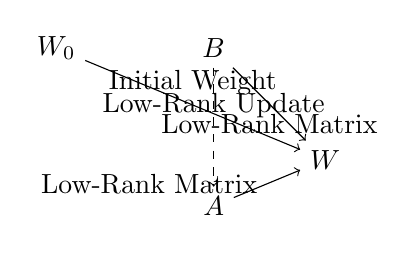
\begin{tikzpicture}[node distance=2cm, auto]

    % Nodes
    \node (W0) {\( W_0 \)};
    \node (B) [right of=W0] {\( B \)};
    \node (A) [below of=B] {\( A \)};
    \node (W) [below right of=W0, xshift=2cm] {\( W \)};
    
    % Arrows
    \draw[->] (W0) -- node[midway, above] {Initial Weight} (W);
    \draw[->] (B) -- node[midway, below] {Low-Rank Matrix} (W);
    \draw[->] (A) -- node[midway, left] {Low-Rank Matrix} (W);
    \draw[dashed, ->] (B) -- node[midway, above] {Low-Rank Update} (A);

\end{tikzpicture}
\end{document}